
\chapter{Introdução}

 \section{Motivação e Lacuna}
 \label{sec:Motivacao}


A aprendizagem profunda (\textit{Deep Learning}) tem se destacado no cenário de Visão Computacional e as Redes Neurais Convolucionais (CNN) \cite{Simonyan14c} tem dominado o estado da arte \cite{ANN}. Estudos podem ser encontrados para detecção de objetos \cite{DBLP:journals/corr/abs-1904-00889, 8437104, 8489369, rs11010011, 8186148}, segmentação de imagens \cite{Zhao2017CVPR,DBLP:journals/corr/CaoSWS16}, contagem de objetos \cite{8186148,DBLP:journals/corr/CaoSWS16,articleLuiz}, entre outros.

Entre as diversas aplicações da Visão Computacional, os métodos de contagem e localização de objetos consistem em detectar e obter a posição de cada objeto individualmente na imagem.
Esses métodos tem auxiliado no controle e contagem de pessoas \cite{ExtractHuman}, carros \cite{CarCount}, animais \cite{8639306}, e até mesmo bactérias \cite{7320116}.
    A maioria dos métodos de contagem são baseados nos mais conhecidos métodos de detecção de objetos (Faster-RCNN \cite{DBLP:journals/corr/Girshick15}, RetinaNet \cite{DBLP:journals/corr/abs-1708-02002}, YoloV3 \cite{DBLP:journals/corr/abs-1804-02767}).
    Esses métodos consideram um retângulo envolvente para cada objeto e podem fornecer tanto a posição (centro do retângulo envolvente) como a contagem (número de retângulos envolventes).

    Embora os métodos recentes tenham obtido resultados promissores, três desafios ainda se mantêm.
    O primeiro desafio é a alta densidade com objetos sobrepostos.
    Em geral, os métodos de detecção de objetos não são adequados para cenários densos de objetos \cite{Goldman2019CVPR}.
    Neste caso, a grande sobreposição dos retângulos envolventes devido a oclusão dificulta o aprendizado dos métodos. Layout Proposal Networks (LPNs) \cite{8237708} é um método recente que tem seguido a proposta de detecção de objetos para contagem de carros utilizando camadas da VGG-16. Seu maior problema na contagem está na sobreposição dos retângulos quando carros estão lado a lado na imagem, como em um estacionamento.


    Por outro lado, estimar um mapa de densidade para obter a quantidade de objetos tem apresentado resultados promissores \cite{DBLP:journals/corr/abs-1808-01050,880968,Cao2017} e  feito com que estudos tenham esta direção.
    Um mapa de densidade consiste em estimar a probabilidade de um objeto ocorrer em cada pixel da imagem.
    Porém a diversidade encontrada nos cenários das imagens (e.g., escala, rotação, etc) dificulta a detecção e contagem por um mapa de densidade. Assim alguns trabalhos buscam encontrar um método eficaz que faça com que o objeto de interesse tenha um destaque nas probabilidades estimadas \cite{inproceedings} \cite{DBLP:journals/corr/abs-1711-04433}.

    O segundo desafio é a necessidade da rotulação detalhada das imagens, o que é difícil de obter em grandes quantidades.
    A rotulação de um retângulo envolvente para cada objeto na imagem torna-se inviável para cenas muito densas em grandes quantidades de imagens.
     Por outro lado, a utilização de um único ponto para rotular cada objeto \cite{8237708} tem sido grande alvo de estudos.
     Por exemplo, \cite{DBLP:peri/corr/abs-1904-01333} propõem o método de detecção e contagem de multidões usando pontos na cabeça das pessoas.
     Os métodos baseados apenas em pontos consideram a informação de contexto ao redor do ponto, pois os objetos compartilham cores, textura e forma.
     Dessa forma, os métodos tendem a reconhecer mesmo que os limites dos objetos não estejam delimitados durante o aprendizado \cite{Aich2018ImprovingOC}.

    O terceiro desafio consiste em contar e localizar objetos em uma sequência de imagens.
   A análise do movimento que objetos realizam nos vídeos podem fornecer informações valiosas que nem sempre são consideradas na contagem de objetos em uma imagem.
Nesse contexto, alguns pesquisadores demonstram em seus estudos que rastrear o movimento pode auxiliar na detecção e reconhecimento, assim como distingui-los do fundo (\cite{Ma_2015_ICCV,Nam_2016_CVPR,Danelljan_2015_ICCV_Workshops,WANG201962,8898173,ExtractHuman}).
   Diferente do rastreamento de objetos, o objetivo deste trabalho é considerar as informações do passado para contar e localizar os objetos em um quadro atual.

    Para contornar os desafios citados acima, este trabalho propõe um método para localizar e contar objetos em vídeos usando redes neurais convolucionais.
    Dado um quadro de um video e o quadro anterior, o método proposto estima uma mapa de densidade com a probabilidade de ocorrência de um objeto em cada pixel.
    Dessa forma, a rotulação apenas de pontos é suficiente para o treinamento do método e cenas densas podem ser melhor modeladas.
    Além disso, o método proposto também estima um mapa de vetores de deslocamento, isto é, vetores que indicam a direção do movimento de cada pixel da imagem.
    Essa estimativa dos vetores de deslocamento também é usada para predizer o mapa de densidade de um quadro atual.
    Todas essa informações são concatenadas para estimar a localização e contagem de objetos do quadro atual.
    Resultados experimentais mostram que a concatenação dessas informações é capaz de melhorar a contagem e localização dos objetos.













\section{Aplicação em Contagem de Peixes}
\label{sec:Aplicação}


O método proposto será aplicado na contagem de peixes e alevinos. Na maioria dos casos, a contagem é um trabalho árduo e requer mão de obra humana atenta, além de ser suscetível a erros.
Por serem sensíveis, os peixes requerem uma afabilidade no manuseio durante a contagem.
Em geral, a contagem acontece por técnicas de barragens \cite{Erikson}, alguns cultivadores realizam a peneiragem para extrair os peixes da água e, dessa maneira, obtêm-se uma estimativa da quantidade de peixes que residem em uma determinada região \cite{OECD,FAO}.


A escada de peixes é uma das maneiras utilizadas na contagem.
Assim os peixes passam por barragens conforme a Figura \ref{fig:escadadepeixes} (a). Na usina hidrelétrica de Igarapava do rio Grande \cite{UHE}, pesquisadores construíram salas (Figura \ref{fig:escadadepeixes} (b)) abaixo do nível d'água, sendo possível enxergar os peixes conforme eles atravessam.
Especialistas na área buscam encontrar técnicas para automatizar a contagem dos peixes que transitam a hidrelétrica.


\begin{figure}[!ht]
	
		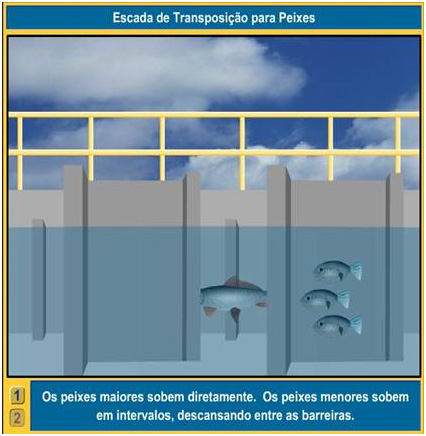
\includegraphics[width=0.4\textwidth]{image/escadadepeixes.jpg}
	    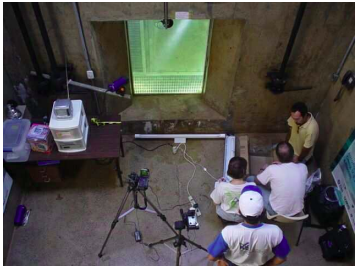
\includegraphics[width=0.55\textwidth]{image/saladaagua.png}
	\caption{(a) Ilustração da Escada de peixes - \cite{UHE}, (b) sala abaixo do nível d'água \cite{Erikson}.}
	\label{fig:escadadepeixes}
\end{figure}

Os cultivadores precisam ter o controle da quantidade de peixes vivos presentes em seus cativeiros, para que a alimentação seja devidamente proporcional para todos, e se há necessidade do cultivo de novos peixes, ou até mesmo alterações no meio. É notória a necessidade de uma exatidão da quantidade que residem uma região.


\section{Objetivos}
\label{sec:objetivos}

\section{Objetivo Geral}
O objetivo deste trabalho é propor um método para contagem de objetos em vídeos utilizando redes neurais convolucionais.
Um dos intentos principais está em detectar tais objetos nas imagens levando em consideração a posição espacial no quadro anterior. Assim com a ciência das localizações anteriormente, uma estimativa mais refinada da posição atual pode ser obtida.


\section{Objetivos Específicos}


Tendo o objetivo geral imposto, os seguintes objetivos específicos foram definidos:
\begin{enumerate}
    \item Estimar a contagem por meio de um mapa de densidade obtido por uma rede neural convolucional;
    \item Avaliar a inclusão do quadro anterior na estimativa do quadro atual;
    \item Incluir vetores de deslocamento na predição do mapa de densidade;
    \item Aplicar o método na contagem de alevinos.

\end{enumerate}








